\structure{ТЕОРЕТИЧЕСКАЯ ЧАСТЬ}

На рисунке \ref{fig:fig01} представлено схематическое изображение источника
акустических колебаний речевого аппарата человека, слухового тракта и
спектрограмма речевого сигнала.

\begin{figure}
    \centering
    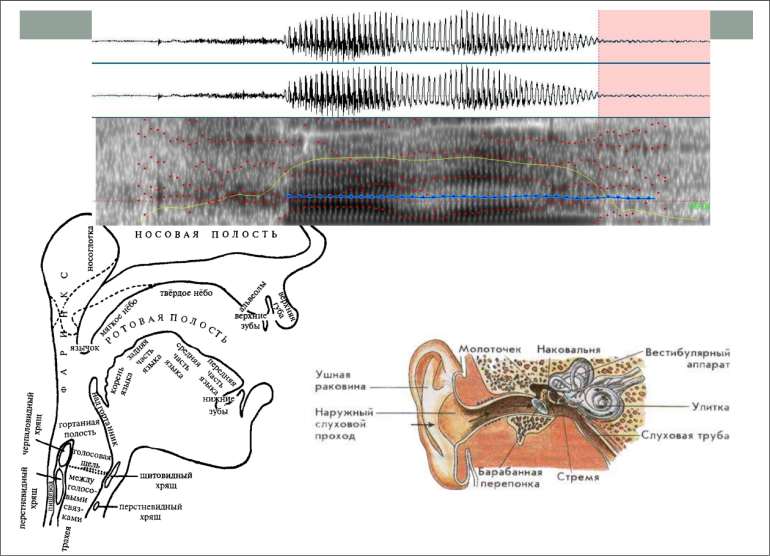
\includegraphics[scale=0.6]{inc/fig_01.png}
    \caption{
        Схематическое изображение источника акустических колебаний речевого
        аппарата человека, слухового тракта и спектрограмма речевого сигнала.
    }
    \label{fig:fig01}
\end{figure}

Речевой аппарат представляет собой неоднородную акустическую трубу, которая
изменяется по форме с течением   времени. Основными анатомическими
компонентами, вызывающими это изменение, являются губы, челюсти, язык и нёбная
занавеска (мягкое нёбо). Например, площадь сечения раскрытия губ может
изменяться от нуля (при закрытых губах) до 20 см² (при опущенной нижней челюсти
и открытых губах). Речевой тракт можно представить в виде простой модели -
линейного фильтра с изменяющимися во времени параметрами, который возбуждается
генератором периодических импульсов белого шума или их совокупности.
Анатомически линейный фильтр формируется акустической трубой, состоящей из
дыхательного (легкие, бронхи, трахея) и произносительного аппаратов (гортань с
голосовыми связками, глотка, носовая и ротовая полости, язык, нёбо, губы).


При разговоре грудная клетка расширяется и сжимается, прокачивая воздух из
лёгких по трахее через голосовую щель. Звуки образуются при выдохе воздуха при
условии, что давление воздуха под голосовыми связками превышает давление над
ними, тогда воздух, проходя через голосовую щель, смыкает и размыкает голосовые
связки, колебания которых модулируют звуковую волну.

Частота смыкания-размыкания связок представляет собой частоту основного тона
речи. Если голосовые связки расслаблены, воздух свободно проходит через
голосовую щель, не подвергаясь модуляции, и речь получается неозвученная. После
голосовых связок воздушный поток проходит через глоточную полость мимо
основания языка и, в зависимости от положения мягкого нёба, через ротовую и
(или) носовую полости, производя при этом шум.  В пространство поток воздуха
излучается в виде акустических волн и, достигнув слухового аппарата человека,
интерпретируется им как речь. Голосовой тракт (и соответствующий ему в модели
речеобразования линейный фильтр) имеет несколько резонансных областей,
создающих энергетически сильные спектральные области - форманты.

Индивидуальные акустические параметры человека определяются уникальными формой
и размерами голосового тракта, свойствами его стенок, динамикой изменения его
геометрии, формой и периодичностью импульсов голосового источника, а также
зависят от взаимодействия носовой и ротовой полостей, анатомических свойств
груди, бронхов, пазух черепа.

Характер изменения формы артикуляторов обусловлен сокращением мышц, управляемых
центральной и периферической нервными системами, которые даже у близнецов,
идеально похожих друг на друга, различаются настолько, что позволяют точно
отличить их друг от друга.

Во время произнесения неназальных звуков нёбная занавеска поднята и отделяет
голосовой тракт от носовой (назальной) полости. Носовая полость представляет
собой дополнительную акустическую трубку Эля передачи звуков, которая
используется при произнесении назальных звуков английского языка $\slash n
\slash$, $\slash m \slash$, $\slash \eta \slash$, например, в словах run, rum,
rung.

Невокализованные звуки, как, например, /f/ в слове fish, произносятся при
ненатянутых голосовых связках путём пропускания через них воздуха, причём
артикулярные органы определяют форму акустической трубы (например, путём
расположения верхних зубов на нижней губе при произнесении слова fish). При
сжатии акустической трубы и колебаниях голосовых связок произносятся
вокализованные фрикативные звуки, такие, например, как /v/ в слове van.
Взрывные звуки (например, /p/, в слове pop) произносятся путём создания
избыточного воздушного давления в области рта с последующим резким спадом после
его раскрытия.


